\documentclass[tikz,border=12pt]{standalone}
\usepackage[utf8]{inputenc}
\usepackage{tikz}
\usetikzlibrary{shapes,arrows.meta,positioning,calc}

\definecolor{ScoutGreen}{HTML}{005432}
\definecolor{ScoutNavy}{HTML}{002855}
\definecolor{ScoutBlue}{HTML}{006EB6}
\definecolor{ScoutRed}{HTML}{A31920}
\definecolor{ScoutAmber}{HTML}{D97706}
\definecolor{BorderGray}{HTML}{CBD5E1}

\begin{document}
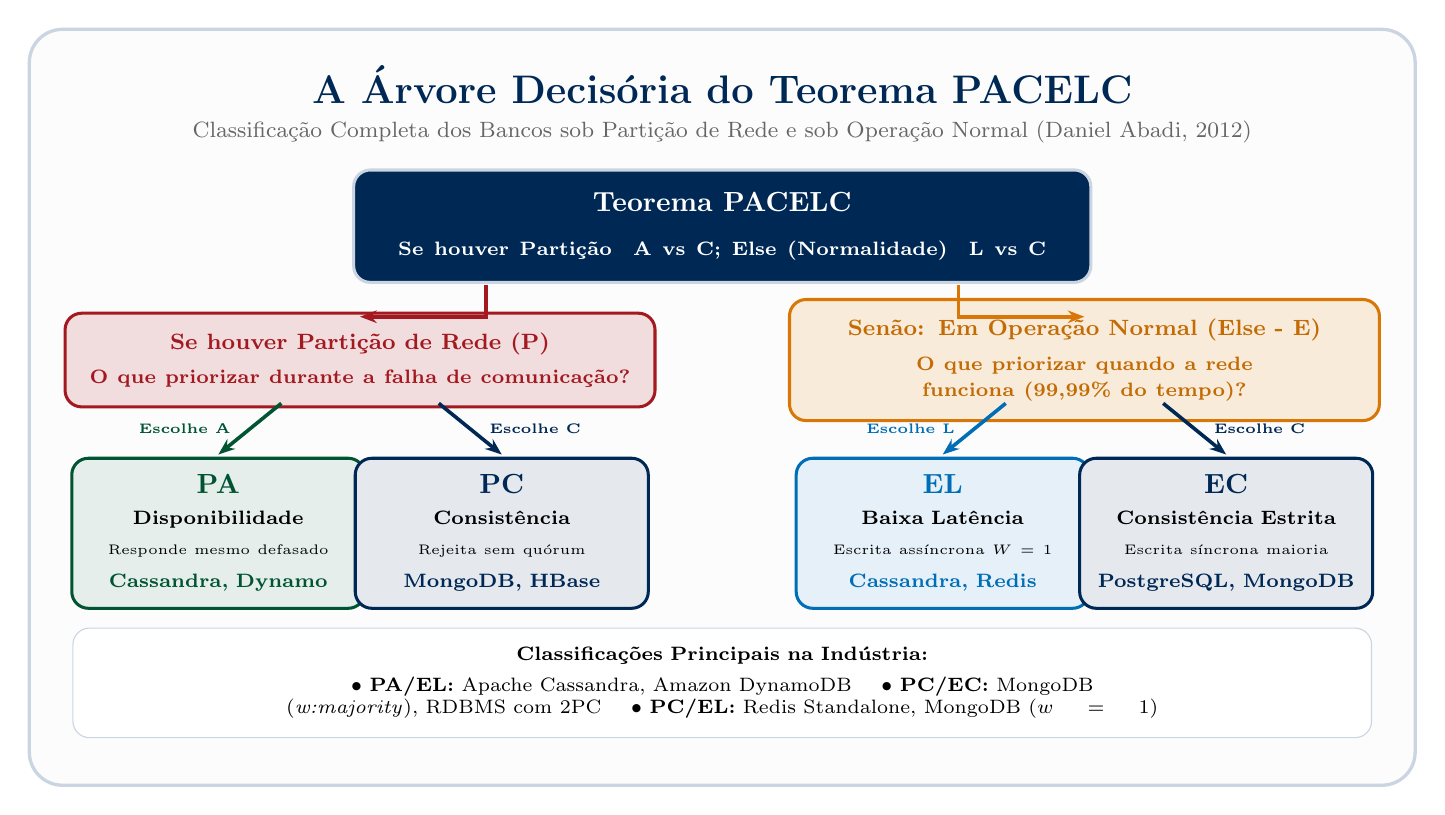
\begin{tikzpicture}[
    font=\sffamily,
    box/.style={draw=BorderGray, rounded corners=6pt, fill=white, line width=1.1pt, align=center, inner sep=6pt},
    arrow/.style={-{Stealth[length=6pt]}, line width=1.3pt}
]

  % Painel Fundo Geral
  \node[draw=BorderGray, rounded corners=12pt, fill=gray!2, line width=1.2pt, minimum width=17.6cm, minimum height=9.6cm] (bg) at (0, 0) {};
  
  \node[font=\bfseries\Large, text=ScoutNavy] at (0, 4.1) {A Árvore Decisória do Teorema PACELC};
  \node[font=\footnotesize, text=gray!80!black] at (0, 3.5) {Classificação Completa dos Bancos sob Partição de Rede e sob Operação Normal (Daniel Abadi, 2012)};

  % Raiz: Teorema PACELC
  \node[box, fill=ScoutNavy, text=white, font=\bfseries\normalsize, text width=8.8cm, inner sep=8pt] (raiz) at (0, 2.3) {
    Teorema PACELC\\[4pt]
    {\scriptsize Se houver \textbf{P}artição $\implies$ \textbf{A} vs \textbf{C}; \textbf{E}lse (Normalidade) $\implies$ \textbf{L} vs \textbf{C}}
  };

  % =========================================================================
  % NÍVEL 1: BIFURCAÇÃO ENTRE PARTIÇÃO (P) E NORMALIDADE (ELSE - E)
  % =========================================================================
  \node[box, fill=ScoutRed!15, draw=ScoutRed, font=\footnotesize\bfseries, text=ScoutRed, text width=7.0cm, inner sep=7pt] (b_part) at (-4.6, 0.6) {
    Se houver Partição de Rede (P)\\[3pt]
    {\scriptsize O que priorizar durante a falha de comunicação?}
  };

  \node[box, fill=ScoutAmber!15, draw=ScoutAmber, font=\footnotesize\bfseries, text=ScoutAmber!90!black, text width=7.0cm, inner sep=7pt] (b_else) at (4.6, 0.6) {
    Senão: Em Operação Normal (Else - E)\\[3pt]
    {\scriptsize O que priorizar quando a rede funciona (99,99\% do tempo)?}
  };

  % Setas saindo limpas da borda inferior da raiz
  \draw[arrow, color=ScoutRed] (-3.0, 1.55) |- (-4.6, 1.15);
  \draw[arrow, color=ScoutAmber] (3.0, 1.55) |- (4.6, 1.15);

  % =========================================================================
  % NÍVEL 2: FOLHAS DECISÓRIAS
  % =========================================================================
  % Sob Partição: PA vs PC
  \node[box, fill=ScoutGreen!10, draw=ScoutGreen, font=\scriptsize, text width=3.3cm, inner sep=6pt] (b_pa) at (-6.4, -1.6) {
    \textbf{\color{ScoutGreen}\normalsize PA}\\[3pt]
    \textbf{Disponibilidade}\\[3pt]
    {\tiny Responde mesmo defasado}\\[4pt]
    \textbf{\color{ScoutGreen}Cassandra, Dynamo}
  };

  \node[box, fill=ScoutNavy!10, draw=ScoutNavy, font=\scriptsize, text width=3.3cm, inner sep=6pt] (b_pc) at (-2.8, -1.6) {
    \textbf{\color{ScoutNavy}\normalsize PC}\\[3pt]
    \textbf{Consistência}\\[3pt]
    {\tiny Rejeita sem quórum}\\[4pt]
    \textbf{\color{ScoutNavy}MongoDB, HBase}
  };

  \draw[arrow, color=ScoutGreen] (-5.6, 0.05) -- (-6.4, -0.6) node[midway, left=3pt, font=\tiny\bfseries, text=ScoutGreen] {Escolhe A};
  \draw[arrow, color=ScoutNavy] (-3.6, 0.05) -- (-2.8, -0.6) node[midway, right=3pt, font=\tiny\bfseries, text=ScoutNavy] {Escolhe C};

  % Sob Normalidade: EL vs EC
  \node[box, fill=ScoutBlue!10, draw=ScoutBlue, font=\scriptsize, text width=3.3cm, inner sep=6pt] (b_el) at (2.8, -1.6) {
    \textbf{\color{ScoutBlue}\normalsize EL}\\[3pt]
    \textbf{Baixa Latência}\\[3pt]
    {\tiny Escrita assíncrona $W=1$}\\[4pt]
    \textbf{\color{ScoutBlue}Cassandra, Redis}
  };

  \node[box, fill=ScoutNavy!10, draw=ScoutNavy, font=\scriptsize, text width=3.3cm, inner sep=6pt] (b_ec) at (6.4, -1.6) {
    \textbf{\color{ScoutNavy}\normalsize EC}\\[3pt]
    \textbf{Consistência Estrita}\\[3pt]
    {\tiny Escrita síncrona maioria}\\[4pt]
    \textbf{\color{ScoutNavy}PostgreSQL, MongoDB}
  };

  \draw[arrow, color=ScoutBlue] (3.6, 0.05) -- (2.8, -0.6) node[midway, left=3pt, font=\tiny\bfseries, text=ScoutBlue] {Escolhe L};
  \draw[arrow, color=ScoutNavy] (5.6, 0.05) -- (6.4, -0.6) node[midway, right=3pt, font=\tiny\bfseries, text=ScoutNavy] {Escolhe C};

  % =========================================================================
  % RESUMO DE CLASSIFICAÇÃO DOS SISTEMAS
  % =========================================================================
  \node[draw=BorderGray, fill=white, rounded corners=6pt, font=\scriptsize, align=center, text width=16.0cm, inner sep=7pt] at (0, -3.5) {
    \textbf{Classificações Principais na Indústria:}\\[3pt]
    $\bullet$ \textbf{PA/EL:} Apache Cassandra, Amazon DynamoDB \quad $\bullet$ \textbf{PC/EC:} MongoDB (\textit{w:majority}), RDBMS com 2PC \quad $\bullet$ \textbf{PC/EL:} Redis Standalone, MongoDB ($w=1$)
  };

\end{tikzpicture}
\end{document}
